\documentclass[a4paper,11pt,oneside]{book}

%\PassOptionsToPackage{table,xcdraw}{xcolor}
% packages 
\usepackage{arsclassica}    % fancy layout
\usepackage[english]{babel}\addto{\captionsenglish}{\renewcommand{\bibname}{References}}
\usepackage{caption}         % figure captions
\usepackage[square,numbers,super,sort&compress]{natbib}  % bibliography style
\usepackage[cc]{titlepic}    % enable logo on title page
\usepackage{graphicx}       % logo related

\usepackage{multirow}

% Margins for pretty version ::
%\usepackage[pass]{geometry}
% Margins for university regulations ::
\usepackage[top=2cm, bottom=4cm, left=4cm, right=2.5cm]{geometry}
\usepackage{setspace}
\onehalfspacing

\usepackage{standalone}
\standalonetrue

\captionsetup{format=plain}

% bibliography
\bibliographystyle{../thesis}

% title setup
\title{ \vspace{3in} Unravelling higher order genome organisation {\small [working
    title]} \\ \vspace{2em} {\large {\bf Results 2} Predictive modelling } }
\author{Benjamin L. Moore}
\titlepic{\vspace{2.2in} 
\includegraphics[width=\textwidth]{/Users/benmoore/hvl/1yrReport/figs/igmm.png}}

\begin{document}

\chapter{Integrative modelling as a tool to explore biological systems}\label{chap:modelling}
\vspace{2em}

\section{Introduction}\label{sec:dongintro}
Large-scale chromatin data has recently been produced by multiple
consortia, most notably ENCODE\cite{Dunham2012} (Section \ref{intro:encode}) but also the NIH
Roadmap Epigenomics project.\cite{Bernstein2010} The breadth and depth of this new
data offers unprecedented opportunities to advance our understanding
of the complex biology of the chromatin landscape. To this end,
studies have already enjoyed success in integrating these data through modelling techniques, with the subsequent dissection of these models revealing novel insights into complex biological phenomena.
%While many histone
%modifications can now be quantified experimentally,\cite{Nikolov2012, Sajan2012, Ernst2011} an integrated
%understanding of general mechanisms underlying the cause or effect of
%these marks lags behind. A 2011 opinion piece asked
%the question ``Histone modification: cause or
%cog?''\cite{Henikoff2011} and speculated that nucleosome modifications
%could be by-products of transcription machinery, as opposed to
%the ``histone code'' hypothesis which suggests that histone
%modifications are placed to direct alterations in chromatin
%state. This latter hypothesis is often tacitly invoked in the
%chromatin literature, wherein a mark may be described as
%``repressive'' or ``activating'' despite only the observation of a
%correlative relationship.\cite{Henikoff2011} 
%Similarly, the interplay
%between locus-level factors and higher-order organisation of
%chromatin, while known the be an important factor in
%transcription, remains poorly understood mechanisatically.\cite{Li2011} 
%and already has provided fascinating new glimpses of the ways chromatin and transcription are functionally related.

Recent studies have shown convincingly that local chromatin state
measurements can accurately predict expression levels of genes on a
genome-wide basis. \citet{Tippmann2012} designed a linear model to predict
steady-state mRNA levels in mouse embryonic stem
cells based on just four predictors: 3 histone modifications
(H3K36me3, H3K4me2 and H3K27me3) and
Pol-II occupancy. Remarkably, the linear model was found to explain
$84.6\%$ of an estimated $91\%$ maximal variance that could be explained
(as calculated through a detailed determination of noise).\cite{Tippmann2012}  An additional
finding of this study was that mRNA half-life and microRNA mediated
transcript degradation both had relatively minor influence on
steady-state mRNA levels, with the authors concluding that ``the lion's
share of regulatory contribution is at the level of mRNA synthesis and
predictable from chromatin alone.''\cite{Tippmann2012} An independent study used a similar regression modelling approach to chromatin
and transcription factor data and again
concluded that models built with histone modifications and chromatin
accessibility data were almost as accurate as those which also
included binding data for 12 transcription factors.\cite{McLeay2012a} 

A recent key study from the ENCODE consortium used ChIP-seq datasets to predict gene expression in a range
of cell types as measured by a variety of experimental techniques.\cite{Dong2012} The authors here developed a
two-stage model which first attempts to classify each transcription
start site (TSS) into an `on' or `off' state using a powerful ensemble
classifier technique called Random Forests (RF). The second stage of the
model used the same range of histone modifications as regressors in a
simple linear modelling framework to quantify predicted
expression. This approach proved very successful, producing a
median Pearson correlation coefficient (PCC) between predicted and
empirical expression levels using 10-fold cross-validation of
$0.83$ across all cell lines and expression level
technologies.\cite{Dong2012} Additionally, this study highlighted cap
analysis of gene expression (CAGE) as the 
technology, relative to RNA-seq and RNA-PET, which produced the most
predictable expression response. CAGE uses 5$^\prime$ capped transcripts to
generate short, specific tags which precisely identify TSS positions as well as
quantifying the abundance of a given transcript.\cite{Shiraki2003, Kodzius2006}

These recent publications highlight the importance and relevance of
advancing our understanding of chromatin biology through a model-based
approach. 
%Each of these existing models however, treats expression
%levels as stationary outcome in each cell type and ignores any temporal
%dynamics. The huge amount of novel timecourse CAGE data 
%produced by the FANTOM5 consortium\cite{fantom5} puts us in an ideal
%position to investigate how chromatin influences transcription beyond a
%simple single-point response and move towards a more complete
%understanding of the drivers of transcriptional flux. 
We can extend this idea to the related domain of nuclear architecture, in the hope of understanding the relationships between chromatin and higher order structure in the same way that chromatin features have been related to transcriptional output.

\section{Extending Dong \emph{et al.} }\label{sec:reprodong}

\begin{figure}
\begin{center}
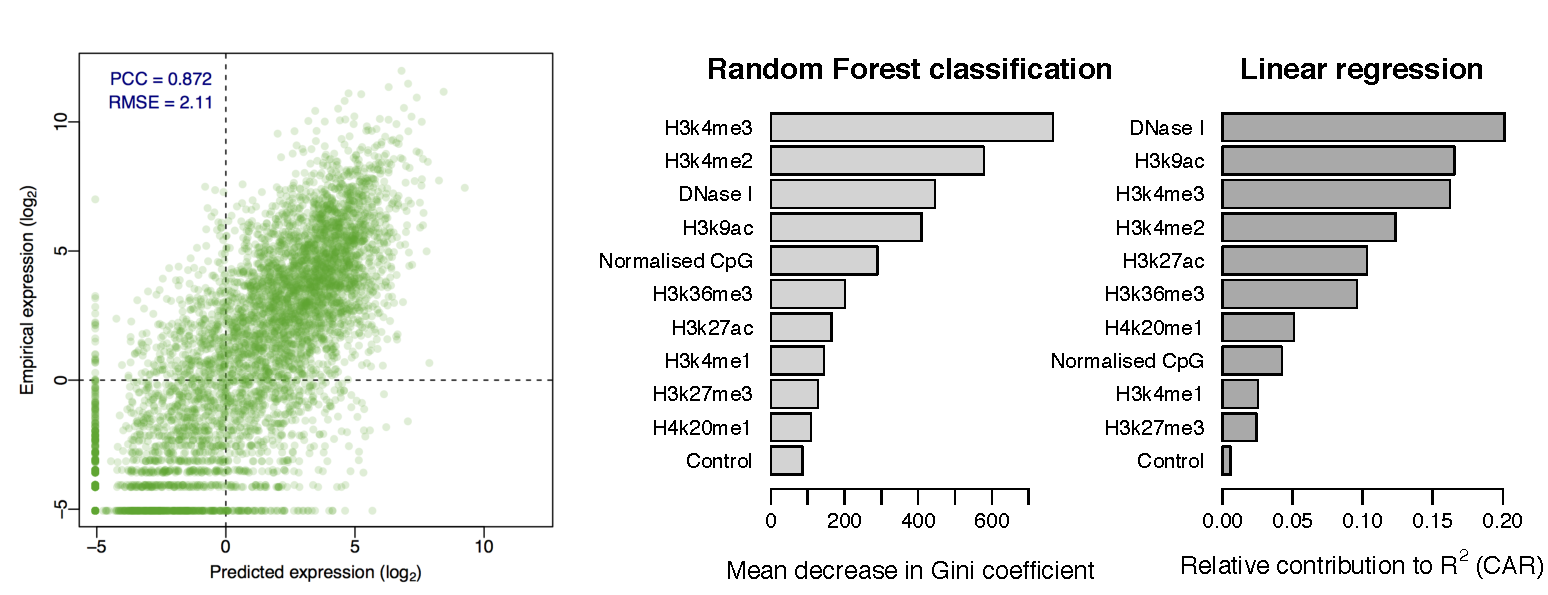
\includegraphics[width=5.65in]{figs/dong_repres.pdf}
\captionsetup{width=\textwidth}
\caption[ Highly accurate models of expression were built following Dong \emph{et al.} ]{ {\bf Highly accurate models of expression were built following Dong \emph{et al.} }  A scatterplot shows the strong correlation between predicted and observed expression levels per transcript (\emph{left}). Variable importance metrics are shown for the on/off RF classification step and continuous linear regression step (\emph{right}). 
}\label{fig:dongres}
\end{center}
\end{figure} 

We reimplemented the published modelling framework of \citet{Dong2012} (introduced in Section \ref{sec:dongintro}) to 
replicate their results and analyse the strengths and caveats of their approach. 

We were able to reproduce the reported results and highly accurate models of transcriptional output. An example is shown for a model of CAGE expression in the H1 hESC cell type (Fig. \ref{fig:dongres}). Note that not all variables used in \citet{Dong2012} were made available for this particular modelling scenario, however the Pearson correlation between predicted and observed expression ($0.87$) is above the study's median value ($0.83$), and in-line with other models predicting CAGE data (median $PCC \approx 0.87$).\cite{Dong2012}

We also re-calculated measures of variable importance for this model of transcription (Fig. \ref{fig:dongres}). We note some small variations from the example model shown in \citet{Dong2012} which was predicting cytosolic CAGE data recorded in K562 cells. This hints at some degree of some variability between cell type models, though broad similarities also exist such as both models ranking DNase I hypersensitivity as a relatively informative variable (Fig. \ref{fig:dongres}).

When replicating the modelling approach of \citet{Dong2012}, we were surprised to find that the two-step classification
then regression (firstly assessing a gene as `on' or `off' and then
predicting its expression level) added little additional accuracy relative to a simple
linear regression model (Fig. \ref{fig:TwoStepvsSimple}). Indeed, it appears the ``best bin`` technique (Section \ref{sec:dongbestbin}) had much greater impact on overall predictive power than the addition of this classification step.

% figure : results of Dong et al. reproduction

\begin{figure}
\begin{center}
\includegraphics[width=4in]{figs/dong_2stepres.png}
\captionsetup{width=\textwidth}
\caption[Comparison of two-step classification-regression model of transcription with
  a simple linear regression model.]{ {\bf Comparison of a published two-step classification-regression model of transcription with
  a simple linear regression model. }  Scatterplots of predicted against empirical
  $\log_2$ reads per million (RPM) expression values for the two-step model of \citet{Dong2012} and simple multiple linear regression are shown (\emph{left})
  along with frequency distributions of predicted and observed
  expression levels (\emph{right}). Scatterplots are annotated with
  Pearson's correlation coefficient (\emph{PCC}) and the root mean
  squared error (RMSE); black trendlines describe $y =
  x$. Overall correlations calculated with 10-fold cross-validation.
}\label{fig:TwoStepvsSimple}
\end{center}
\end{figure} 

\subsection{\emph{Bestbin} method}\label{sec:dongbestbin}
An innovative element of the modelling approach used in \citet{Dong2012} is the `bestbin' method of matching
chromatin measurements to the expression of a given TSS. This strategy
first bins normalised signal intensities into $40 \times 100$ bp bins
encompassing 4 kb around the TSS, and adds an additional bin representing the remaining
gene body. Then the correlation between
the signal of a given mark and the expression of a TSS across all
genes is measured, then the bin producing the highest correlation is
designated as the `bestbin' and that bin's normalised ChIP-seq signal intensity is
taken forward for the full model. This was shown to raise
the correlation (between predicted and observed expression) by $0.1$ in
the simple regression model, an increase in accuracy of almost $13\%$,
relative to simply taking the average value across all
bins.\cite{Dong2012} 

\begin{figure}
\begin{center}
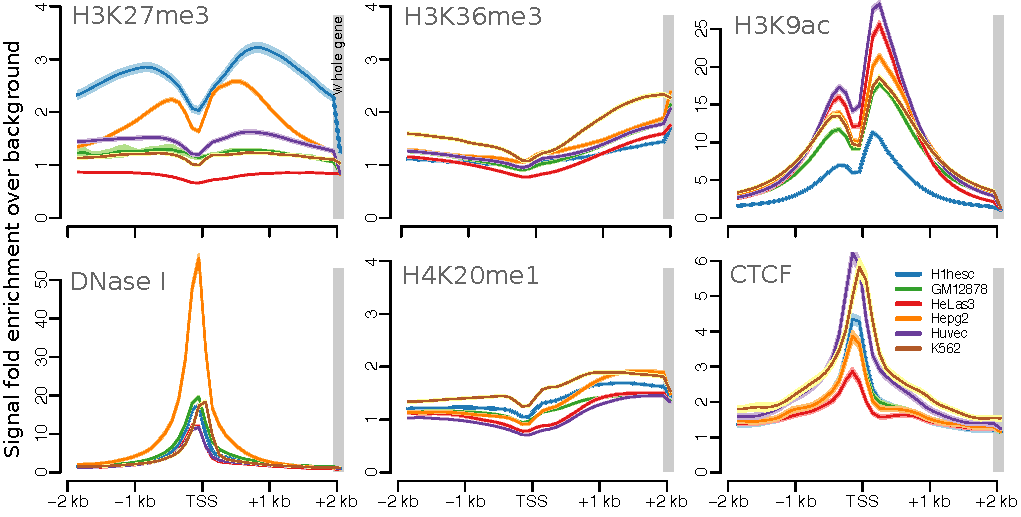
\includegraphics[width=5.3in]{figs/dong_tss_profiles.pdf}
\captionsetup{width=\textwidth}
\caption[ Average input feature profiles over transcription start sites. ]{ {\bf Average input feature profiles over transcription start sites. }  Mean ChIP-seq signal over input control is shown for 6 factors in 6 human cell types used in \citet{Dong2012}. Each is averaged genome-wide over GENCODE v7 \texttt{hg19} defined TSS $\pm 2$ kb, and over whole genes (\emph{grey shading}). Ribbons shown $99\%$ confidence intervals of the mean. 
}\label{fig:dongtssprof}
\end{center}
\end{figure} 

The justification for such an approach hinges on the idea that the multitude of input features (mostly histone modifications and DNA binding proteins) have a variety of biological functions, and so the bestbin method is one way of learning these functions in an automated and unsupervised way. For example, the histone modification H3K36me3 is understood to be painted across exons that are being actively-transcribed,\cite{Tippmann2012, Kolasinska-Zwierz2009, Schaft2003} thus the genome-wide summary statistic that best captures this function is likely the whole-gene measurement, rather than the level of H3k36me3 at a gene's TSS or upstream promoter. A re-analysis of ENCODE data used in \citet{Dong2012} highlights this kind of variability across input features (Fig. \ref{fig:dongtssprof}). Some marks clearly are enriched directly over TSS (CTCF, DNase; Fig. \ref{fig:dongtssprof}) while others show enrichments along the gene body (H3K36me3, H4K20me1; Fi.g \ref{fig:dongtssprof}) as well as more-complex, asymmetrical "shoulder" patterns (H3K27me3, H3K9ac; Fig. \ref{fig:dongtssprof}). Bestbin will therefore, to some degree, capture these spatial relationships without \emph{a priori} specification.

% Dissection of best bin (bestbinDetermination.pdf ?)

%\subsection{Variable importance}

\begin{figure}
\begin{center}
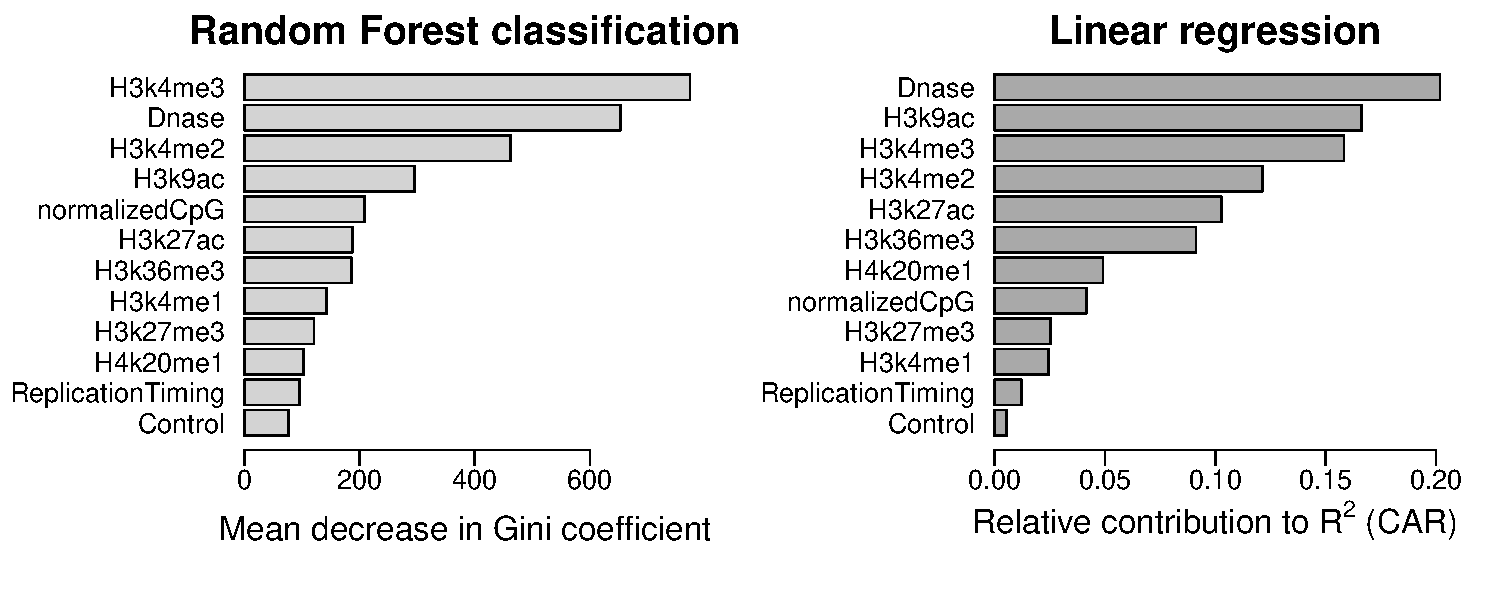
\includegraphics[width=\textwidth]{figs/Dong_relImp_Horiz.pdf}
\captionsetup{width=.9\textwidth}
\caption[Relative importance metrics for variables in both stages of a reimplementation of a published model for predicting transcriptional output.]{ {\bf Relative importance metrics for variables in both stages of a reimplementation of a published model for predicting transcriptional output. } 
Variable importance is measure by decrease in Gini coefficient for the RF classification step, and by CAR $R^2$ decomposition\cite{Zuber2011} for the linear regression step.
}\label{fig:relimp}
\end{center} 
\end{figure} 

\subsection{Model adjustments}

We attempted to improve the accuracy of predicted expression values
produced by \citet{Dong2012} through increasing the number of informative
regressors. While \citet{Dong2012} included broad coverage of different histone modifications,
they did not investigate the impact of higher order
chromatin data. For this reason, we matched the TSS positions used in
\citet{Dong2012} with previously-published genome-wide replication
timing ratios measured in BG02 ESCs.\cite{Ryba2010} This data is of a different origin to the transcriptional data in this case (which was record in H1 hESC) but replication timing is thought to be largely conserved between cell types.\cite{Chambers2013} 

We then used these values as an additional
regressor in both the two-step classification regression model and the
simple linear model but saw no significant improvement in either
model's accuracy (\emph{data not shown}). The reasons for this are likely that the 
data were relatively low-resolution (1 Mb), from a
imperfectly matched cell line and also that
the existing model is already achieving such accurate
results that they must already be accounting for most of the maximal
explainable variance in gene expression given experimental and
biological noise. With this in mind, additional regressors would be
expected to yield diminishing returns. Even so, on closer examination,
the replication timing data
appeared only slightly more informative than the control ChIP-seq input
measurements when evaluated with relative importance metrics
(Fig. \ref{fig:relimp}), implying that large-scale chromatin domains
and do not have significant influence on the expression of the genes resident within them. 

\section{Modelling FANTOM5 expression data}

Using FANTOM5 CAGE data\cite{fantom5} and the approach established above (Section \ref{sec:reprodong}), we next attempted to model gene
expression at timepoint zero ($t_0$) of a differentiation timecourse of Human
H1 embryonic stem cells (H1 hESC) to CD34+ hematopoietic stem
cells. Applying this modelling strategy to a novel dataset will allow us to assess the portability of the model design, as well as permitting more detailed breakdown of model components, such as the bestbin strategy.

% How did I do this?:
% 1) Take robustly mapped CAGE clusters -> Entrez Gene IDs
% 2) Select the strongest expressed CAGE cluster
% 3) Either a) use this as a TSS or b) map to closest annotated TSS
%The first stage of the analysis was to map each CAGE cluster to a
%representative TSS. FANTOM5 robust gene mapping\cite{fantom5}
%provided corresponding Entrez Gene IDs for gene-associated CAGE
%clusters, and we selected the most expressed cluster to represent the
%expression level of its mapped gene. We then compared these to Ensembl
%TSS annotations (v69) and
%discarded those tag clusters centered on a point $>50$ bp from an annotated
%TSS associated with the mapped Entrez Gene ID, thereby removing enhancers and other non-genic transcribed
%regions.

We retrieved a number of genome-wide ChIP-seq datasets measured in H1 hESC cells and produced by the ENCODE consortium\cite{Dunham2012} (Methods \ref{meth:fantom5}). These were matched to transcript annotations to build an input feature set for use in building a predictive model of transcriptional output.

Due to the finding that a two-step (classification--regression) approach added little additional modelling accuracy (Fig. \ref{fig:TwoStepvsSimple}), we employed a single-step design using a Random Forest (RF) regression model.\cite{Breiman2001, Diaz2006} With a total of 14 predictors (10 histone modifications, HDAC6, H2A.Z, DNase I and an input control, listed in Methods \ref{meth:fantom5}), we were able to build a highly accurate predictive model of transcriptional output of around $11,000$ TSS (Fig. \ref{fig:model}).

\begin{figure}
\begin{center} 
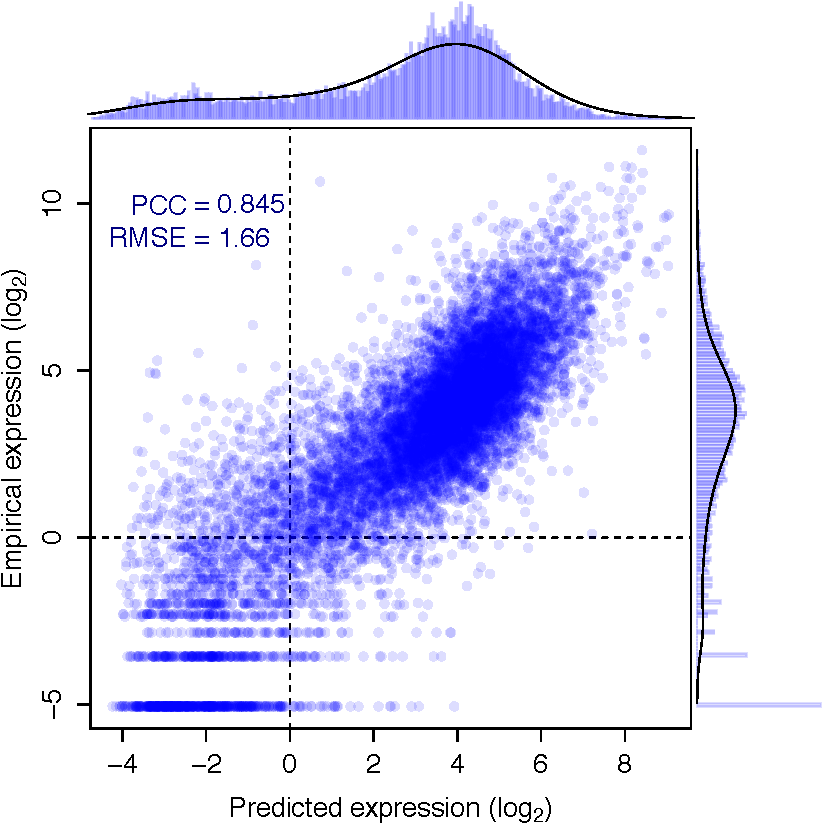
\includegraphics[width=.6\textwidth]{figs/RandomForest_10CV_50d.pdf}
\captionsetup{width=\textwidth} 
\caption[Random Forest predictions of FANTOM5 expression data.]{ {\bf Random Forest predictions of FANTOM5 expression data. } RF model predictions are plotted against their empirical values. The marginal distributions of predicted and empirical
  expression values are shown opposite their
  respective axes. Pearson's correlation coefficient ($r$) and the root
  mean-squared error (RMSE) are shown (\emph{inset}).
}\label{fig:model}
\end{center} 
\end{figure} 

Model predictions evaluated with 10-fold cross validation show a
highly significant correlation with measured CAGE levels ($PCC = 0.845\pm
1 \times 10^{-4}$, $p < 2 \times 10^{-15}$), and the model is able to explain around
$71\%$ of the variance in the expression response (for comparison a
linear model resulted in $PCC = 0.825 \pm 3.2 \times 10^{-5}$, $p < 2 \times 10^{-15}$). This result is worse than that of \citet{Dong2012}
who achieved cross-validated correlation coefficients of up to $0.9$,
but it is roughly equal to their median test set correlation of
$0.83$.\cite{Dong2012}  However the RMSEs of our predictions, when normalised by the range of
observed values, compare more favourably ($0.11$, compared with Dong \emph{et al.}'s: $0.14$). 

Our slightly lower predictive power could be explained by our streamlined model design. \citet{Dong2012} implemented a pseudocount optimisation step whereby an additional count added to each binned signal
intensity prior to log transformation to maximise expression correlation. In the model presented above, a fixed
pseudocount of $1$ was used to avoid introducing an unwarranted positive bias towards higher correlation. We confirmed that a two-step classification--regression design did not improve our model performance metrics; indeed, the PCC and RMSE of a classification--regression framework with this data showed a slight decrease in prediction accuracy ($PCC = 0.834 \pm 0.007$, $\textrm{RMSE} = 1.77$ when applied to the same test and
training data used in Fig. \ref{fig:model}).

%A possible explanation for our lower modelling accuracy relative to that of \citet{Dong2012} is that in our case, while both chromatin data and expression were measured in H1 hESC cells, the experiments took place at
%different institutes using unstandardised protocols and cell cultures. For comparison, a previous study using chromatin
%measurements from a number of different sources to predict expression
%in a matched cell-type reported a predictive correlation of 0.77.\cite{Karlic2010} The ENCODE consortium, on the other hand, went to some lengths to standardise protocols and minimise batch effects between samples.\cite{Dunham2012} 

\subsection{\emph{Bestbin} analysis}

We again implemented the previously-described `bestbin' strategy\cite{Dong2012} (Section \ref{sec:dongbestbin}) to objectively
select the most-correlated binned signal for each chromatin H1 hESC
mark. To explore the implications of this approach, we analysed the stability of chosen bestbins by
calculating them on $200$ sets of $1000$ randomly selected TSS samples, with each sample
representing approximately $8\%$ of the complete dataset. Distributions of chosen bestbins across these 200 sub-samples are shown as boxplots (Fig. \ref{fig:bestbin}).

\begin{figure}
\begin{center} 
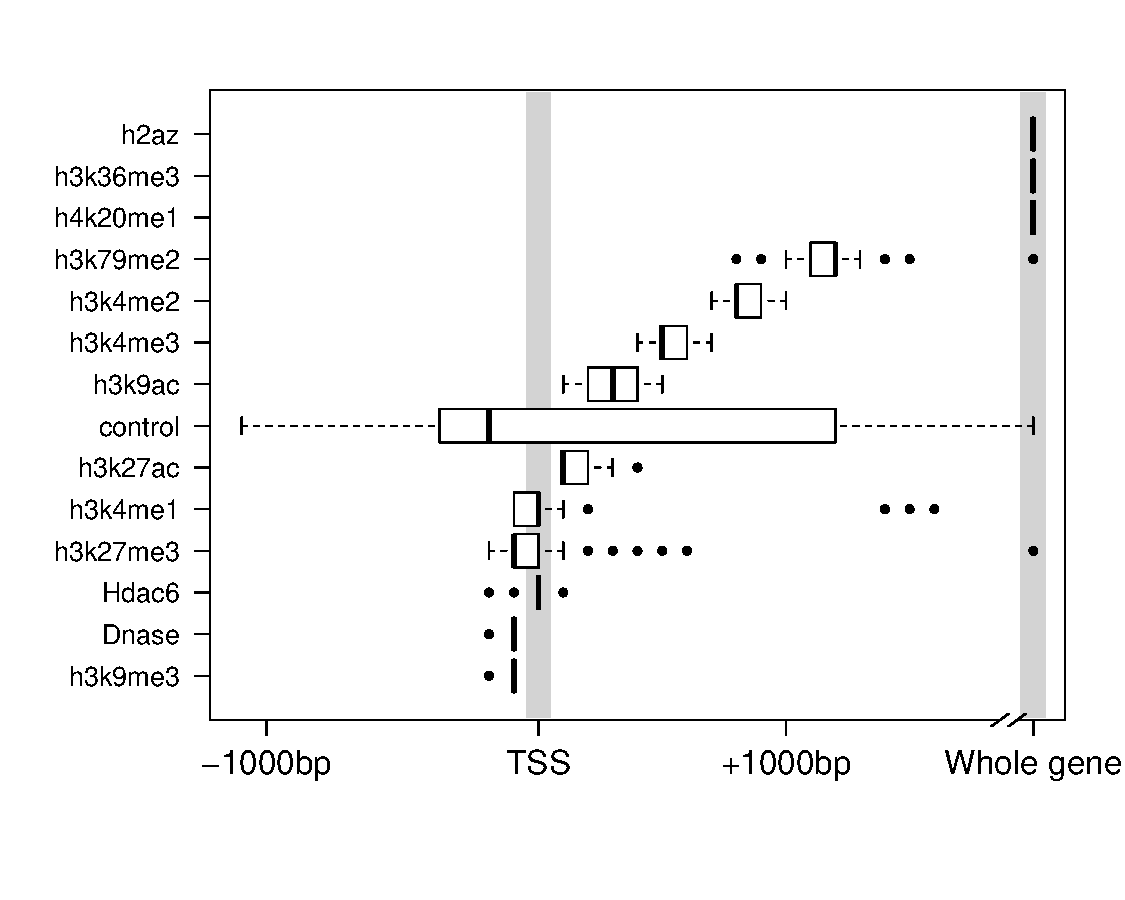
\includegraphics[width=4.5in]{figs/bestbinSummary.pdf}
\captionsetup{width=\textwidth}
\caption[Distributions of bestbin locations relative to the
  TSS.]{ {\bf Distributions of bestbin locations relative to the
  TSS.} Bestbins were selected for normalised ChIP-seq
  signal intensities for 10 histone marks, the
  H2A.Z histone variant, Hdac6 histone deacetylase, DNase
  hypersensitivity and a ChIP-seq input chromatin control. Bins analysed
  extended 2 kb flanking the TSS, but more distal bins were
  never selected and hence are not shown. `Whole gene` represents the
  averaged signal intensity from TSS to transcript end site, as
  defined by Ensembl Genes v69.
}\label{fig:bestbin}
\end{center}
\end{figure} 

We find that bestbin selections are often highly consistent across sub-samples, indicating there are fairly static informative regions relative to a TSS for each chromatin factor. Furthermore, the selected
bestbins match known biological mechanisms; for example the H3K36me3
mark's bestbin is consistently the whole gene measurement (Fig. \ref{fig:bestbin}) and this
mark is known to be enriched in actively transcribed
exons.\cite{Tippmann2012, Kolasinska-Zwierz2009, Schaft2003} The negative control variable (ChIP-seq input) shows no strong location bias, as expected (Fig. \ref{fig:bestbin}). Other distributions are less easily explained, such as those features showing a tight distribution of informative regions slightly downstream of the TSS (H3K9ac, H4Kme2/3 and H3K79me2; Fig. \ref{fig:bestbin}).


% Cut out timecourse stuff?

%Having built a reasonable model of $t_0$ expression, the next stage of
%this preliminary analysis was to consider successive timepoints. In the
%available CD34+ differentiation dataset, this consisted of expression
%data recorded at three
%timepoints (days 0, 3 and 9---hereafter $t_0$, $t_3$ and $t_9$
%respectively). However genome-wide expression
%was highly correlated between each of these timepoints (Pearson correlation coefficients: $t_0, t_3 = 0.911; ~t_0,t_9 =
%0.913; ~t_3,t_9 = 0.977$), and this high correlation meant that the
%genome-wide model performed essentially equally well regardless of the
%expression timepoint it was trained or tested on. In future analyses, higher-resolution timecourses may offer
%more interesting variation or alternatively genes that remain invariant
%throughout the timecourse could be filtered out of the dataset. 

\section{Modelling higher order chromatin}\label{sec:modhoc}

Accurate predictive modelling of transcription in a variety of cell types offered several novel insights into the interrelationships between locus-level chromatin features and transcriptional machinery, as well as advancing a quantitative explanation of the degree to which correlated features are informative. It is of interest then, to test whether this approach can be applied to other data, such as the reprocessed higher order chromatin organisation data assembled in this work (Chapter \ref{chap:hiccomparison}).

Previous publications have identified several correlates which track compartment eigenvector profiles to varying degrees,\cite{Lieberman2009, Imakaev2012} yet to date these relationships have not been quantitively investigated. The above-described modelling framework offers a statistical approach towards understanding the drivers of these observed correlations.

\subsection{Predictive model}

We built Random Forest regression models (Methods \ref{sec:rf}) to predict compartment eigenvector profiles genome-wide in three human cell types. Models were found to have high predictive accuracy, with Pearson correlation between predicted and observed compartment eigenvectors in the range of $0.82$--$0.75$ (Fig. \ref{fig:modelres}), comparable to that achieved by \citet{Dong2012} in the prediction of transcription.

\begin{figure}
\begin{center} 
\makebox[\textwidth][c]{ 
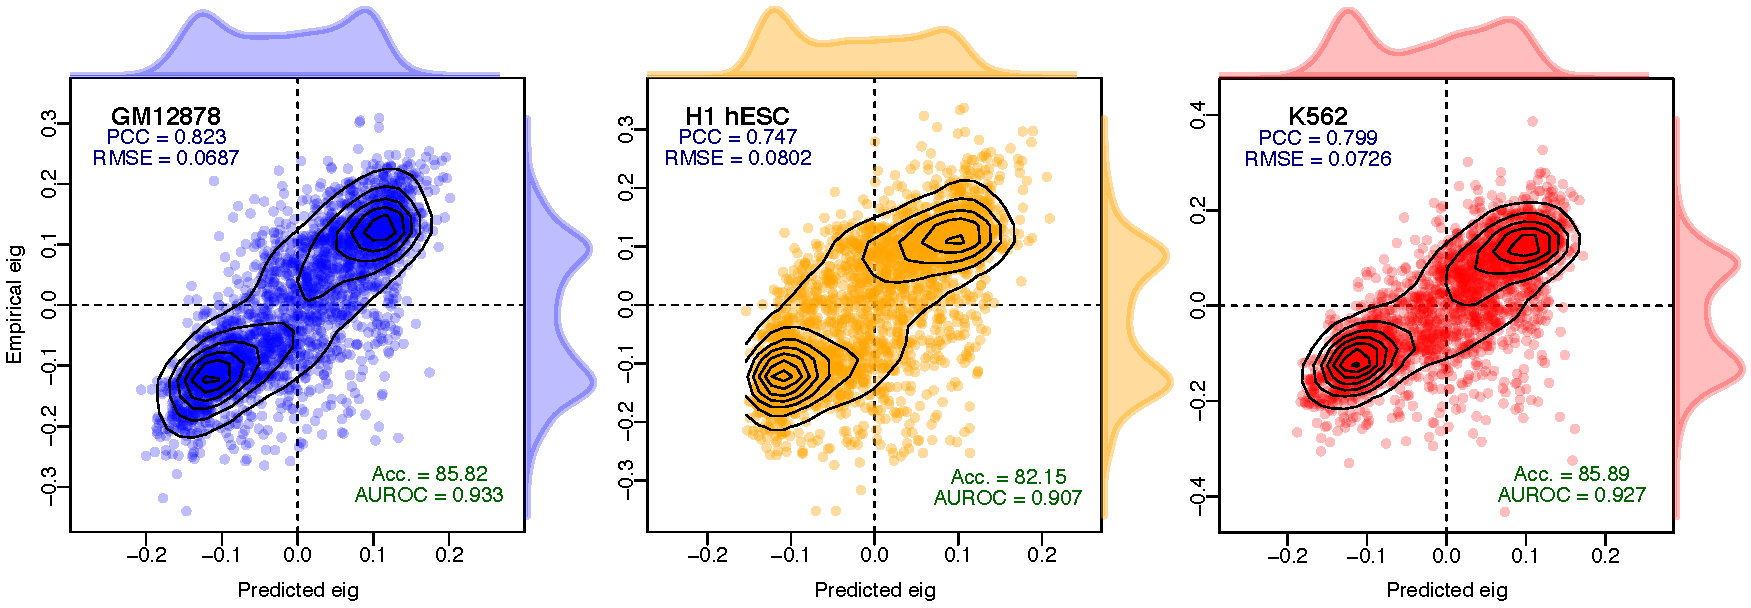
\includegraphics[width=1.1\textwidth]{figs/modelres.pdf}
}
\captionsetup{width=\textwidth} 
\caption[Compartment eigenvector model predictions are highly correlated with observed values.]{ {\bf Compartment eigenvector model predictions are highly correlated with observed values.}  Pearson correlation coefficient (PCC) and root mean-squared error (RMSE) report the degree of success of the regression model, whereas accuracy (Acc.) and area under the receiver operating characteristic (AUROC) give the classification accuracy of binarized outcomes.
}\label{fig:modelres}
\end{center} 
\end{figure} 

Our predictive models were also assessed in terms of classification performance, i.e. did the model correctly assign each block to an A or  B compartment. Instead of retraining a classifier and building parallel models, instead for an estimate of classification accuracy we threshold our regression predictions (Methods \ref{sec:modelperf}). We found our Random Forest models achieved high classification accuracy with $\geq82\%$ of all $1$ Mb genomic bins correctly assigned in each cell type (Fig. \ref{fig:modelres}). 

This predictive performance underlines the strong connection between locus-level features and higher order chromatin structure previously noted by \citet{Lieberman2009} Given such highly-predictive models can be generated, it is then of interest to dissect said models in an attempt to understand the nature of this captured relationship.

% Model showing actual predictions? ala: http://journals.plos.org/ploscompbiol/article?id=10.1371/journal.pcbi.1003419

\subsection{Cross-application}

High predictive accuracy on cell type specific models could be the result of ``over-fitting". In machine-learning, over-fitting refers to the point at which parameters are being optimised to capture noise within a feature set, as well as signal, thereby giving an overoptimistic model performance which would not generalise to another featureset with different noise profiles.

To test if over-fitting was causing our high observed accuracy, we cross-applied models learnt in one cell type to unseen input data from each of the other two cell types under study. If predictive accuracy is a lot lower on unseen data, this lends evidence to the idea that our models may be overfit to their respective cell types. Conversely, it could be the case that biologically-distinct mechanisms are in place that differ between cell types, preventing a simple cross-application.

\begin{figure}
\begin{center} 
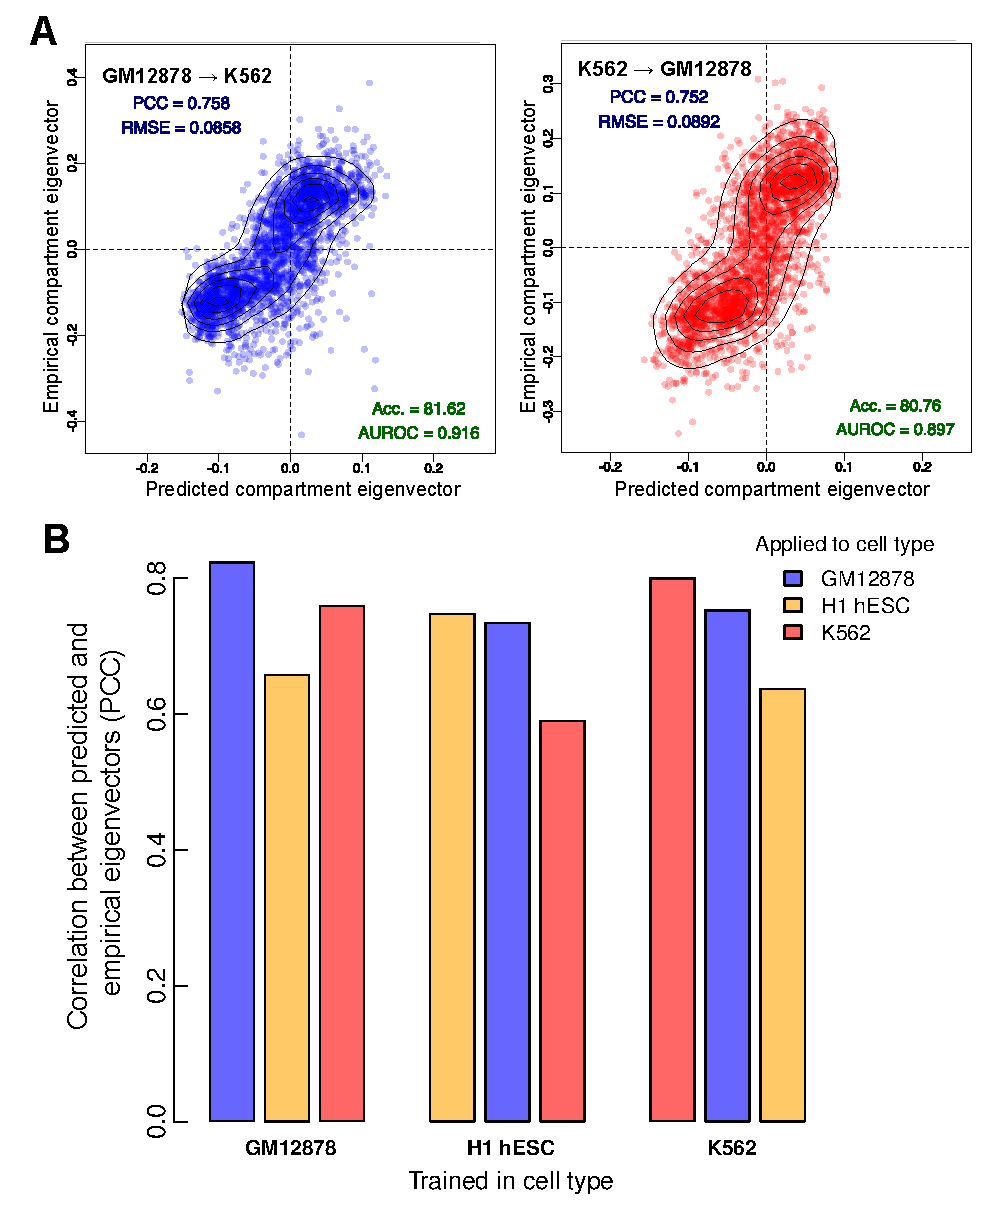
\includegraphics[width=3.5in]{figs/xapp.pdf}
\captionsetup{width=\textwidth} 
\caption[ Models of higher order chromatin structure learned in one cell type can be cross-applied to others.]{ {\bf Models of higher order chromatin structure learned in one cell type can be cross-applied to others. }
 Each model, trained in one cell type, was applied to the chromatin feature datasets from the other two cell types. (A) The GM12878 model achieved high accuracy when applied to K562 features (PCC $= 0.76$), as did the reciprocal cross (PCC $= 0.75$). (B) In each case, predictive accuracy decreased on cross-application but there remains significant agreement between predicted and empirical values. Acc., accuracy; AUROC, area under the receiver operating characteristic curve; PCC, Pearson correlation coefficient; RMSE, root mean-squared error.
}\label{fig:xapp}
\end{center} 
\end{figure} 

We found cross-application between cell types was possible and resulted in similarly-high levels of accuracy to within cell-type cross-validation (Fig. \ref{fig:xapp}). This gives good evidence not only that are models are not overfitting to cell-type specific noise, but also that there exist broad rules linking chromatin conformation and locus-level feature aggregation. The cross-application suggests there exists enough commonalities for compartment profile predictions to transcend the cell-type specific biology inherent to an embryonic stem cell or differentiated lymphoblast.

\subsection{Between-cell variability}
 
\begin{figure}
\begin{center} 
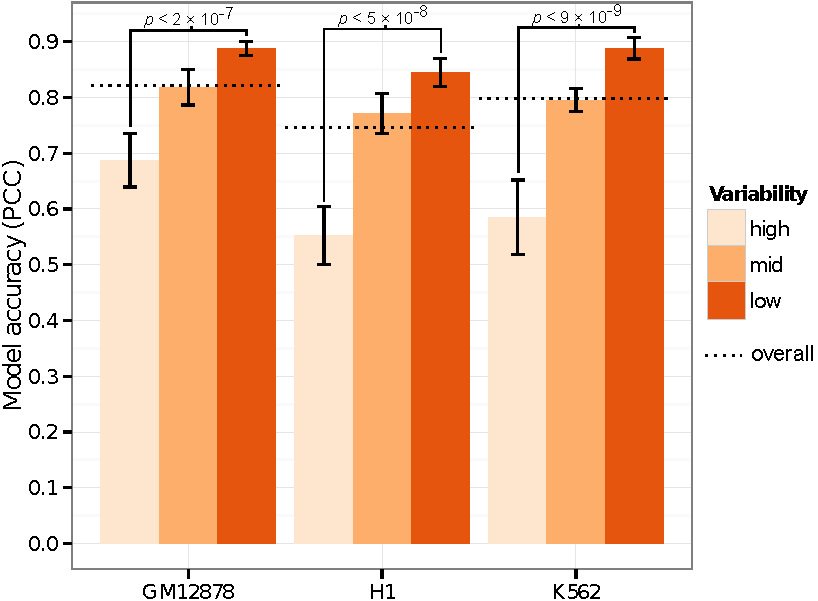
\includegraphics[width=3.5in]{figs/stratmod.pdf}
\captionsetup{width=\textwidth} 
\caption[Genomic regions that vary across cell types are modelled less successfully than static regions.]{ {\bf Genomic regions that vary across cell types are modelled less successfully than static regions. }
Genome-wide compartment eigenvectors were partitioned into thirds according to their median absolute deviation (MAD) across the three cell types under study. Models were fit independently to each third, and the modelling accuracy is compared.
}\label{fig:stratmod}
\end{center} 
\end{figure} 
 
Given much of the higher order chromatin organisation is conserved between the three cell types used in this work (Fig. \ref{fig:compcor}), a testable hypothesis is that these conserved regions are drivers of cross-applicability between cell types. Conversely, genomic regions which vary most across the cell types in our dataset should be more difficult to predict.

Indeed we found the most variable regions across cell types were then most difficult to predict through our Random Forest modelling framework (Fig. \ref{fig:stratmod}). In each cell type, the third of the genome with the most consistent compartment eigenvectors across cell types could then most accurately be modelled in each cell type, and conversely the most variable third shown significantly depleted predictability (Fig. \ref{fig:stratmod}). This latter result suggests these variable regions could either be those which are noisiest, where the eigenvector is least capturing compartment structure, or where cell-type specific biology is influencing compartment structure in ways not captured by our input feature set and low resolution modelling pipeline.

\subsection{Variable importance}

\begin{figure}
\begin{center} 
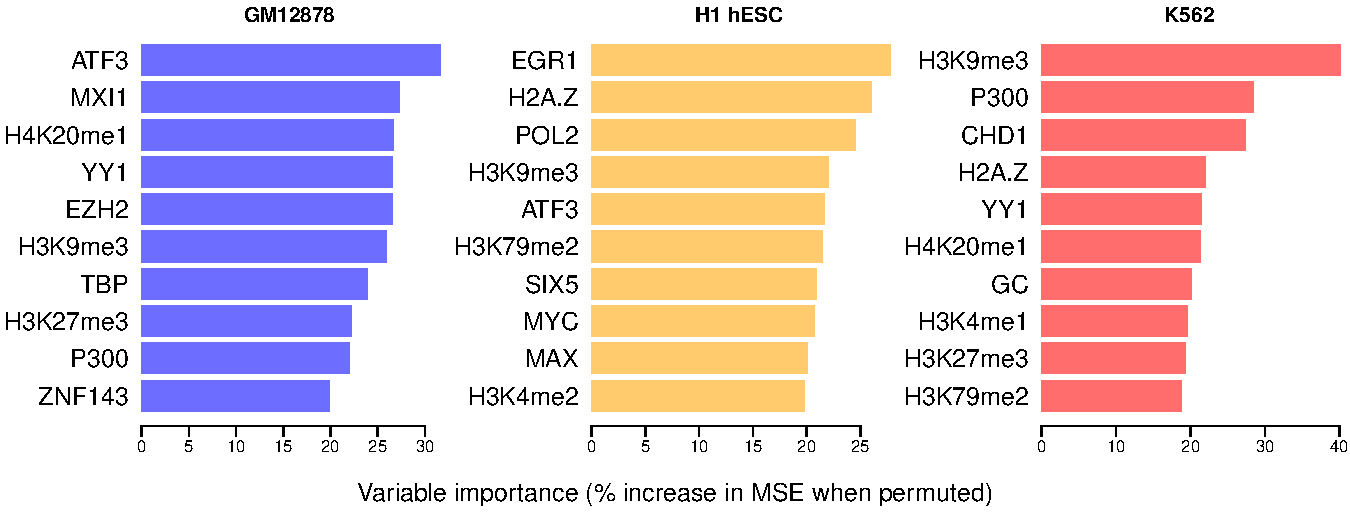
\includegraphics[width=\textwidth]{figs/varimp.pdf}
\captionsetup{width=\textwidth} 
\caption[Variable importance per cell type specific model.]{ {\bf Variable importance per cell type specific model. }
Variable importance for each Random Forest model was measured in terms of percentage increase in mean squared error when permuted (Methods \ref{sec:rf}) and the top 10 ranking variables are shown for each model.
}\label{fig:varimp}
\end{center} 
\end{figure} 

Having built accurate predictive models, we next dissect the relative variable contributions made from our range of input features and compare these across cell types. An overview on the top 10 most highly-ranked features in cell type specific models shows some agreement but also substantial differences between cell types (Fig. \ref{fig:varimp})

Only one input feature, H3k9me3, is present in the top 10 most important variables of each model (Fig. \ref{fig:top10venn}). H3k9me3 is one of the few features to be negatively correlated with compartment eigenvectors (e.g. Fig. \ref{fig:h1feats}). Of those shared between two cell type models, H3k27me3 is also a repressive mark and deposited by polycomb repressive complex 2 (PRC2)\cite{Vizan2014} while H2A.Z is a histone variant again linked to polycomb-regulated genes and essential for embryonic development.\cite{Creyghton2008} Furthermore EZH2, the catalytic subunit of PRC2,\cite{Deb2014} is also included in the feature set but only highly ranked in the GM12878 cell type model. As another example, MYC and MAX are found in the top 10 influential variables in H1 hESC, while MXI1 is found to be an informative variable in GM12878. This is in keeping with recent results suggesting MYC
binds open chromatin as a transcriptional amplifier in embryonic stem
cells,\cite{Nie2012, Kieffer-Kwon2013a} with MAX and MXI1 long being
known as antagonistic co-regulators of MYC.\cite{Zervos1993} These biological relationships between variables may help explain the observed differences between models: different representatives of correlated clusters of input variables may be being selected in each model (see Section \ref{sec:corrinputs}).

\begin{figure}
\begin{center} 
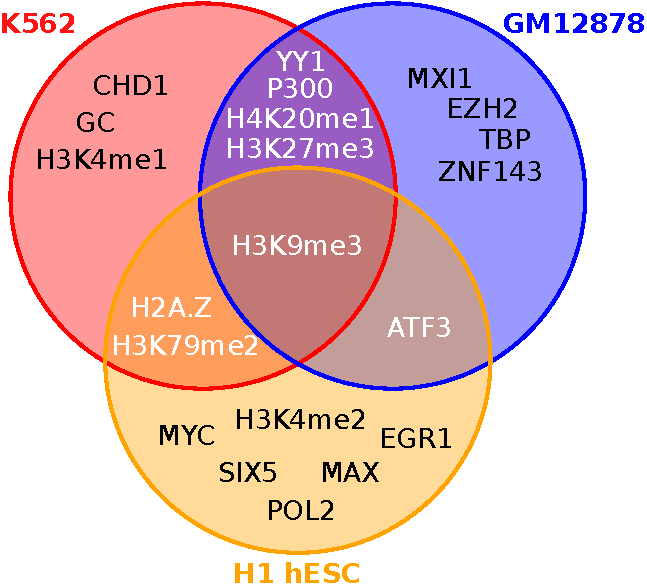
\includegraphics[width=.5\textwidth]{figs/top10venn.pdf}
\captionsetup{width=\textwidth} 
\caption[Intersections of the top 10 ranked variables in the cell type specific models.]{ {\bf Intersections of the top 10 ranked variables in the cell type specific models. }
Venn diagram illustrating intersections between sets of ten most influential variables per cell type specific Random Forest regression model of compartment eigenvector (Fig. \ref{fig:varimp}).
}\label{fig:top10venn}
\end{center} 
\end{figure} 

To assess the significance of observed intersections (Fig. \ref{fig:top10venn}), the variable selection process could be modelled with, for example, a multivariate hypergeometric distribution or via simulation. Simulation was used here for simplicity: each intersection was calculated under $10,000$ variables draws with uniform distribution and empirical $p$-values were then calculated accordingly. Under the assumption that variables are ranked independently in each cell type, drawing at least one variable in all three cell types would be expected by chance ($p = 0.6$). Similarly, the overlaps between pairs of cell types is within the range of expectation (probability of 7 or more variables appearing in exactly two sets: $0.39$). Hence these data suggest the top 10 most influential variables are not significantly more alike across the three cell-type specific models than expected by chance, however ten is an arbitrary cutoff, and many of the rankings are based on small differences in variable importance, thus could be unstable between multiple generations of stochastic Random Forest models.

% figure showing e.g. how individual var regresses against eigen (Egr1compare.pdf)
\begin{figure}
\begin{center} 
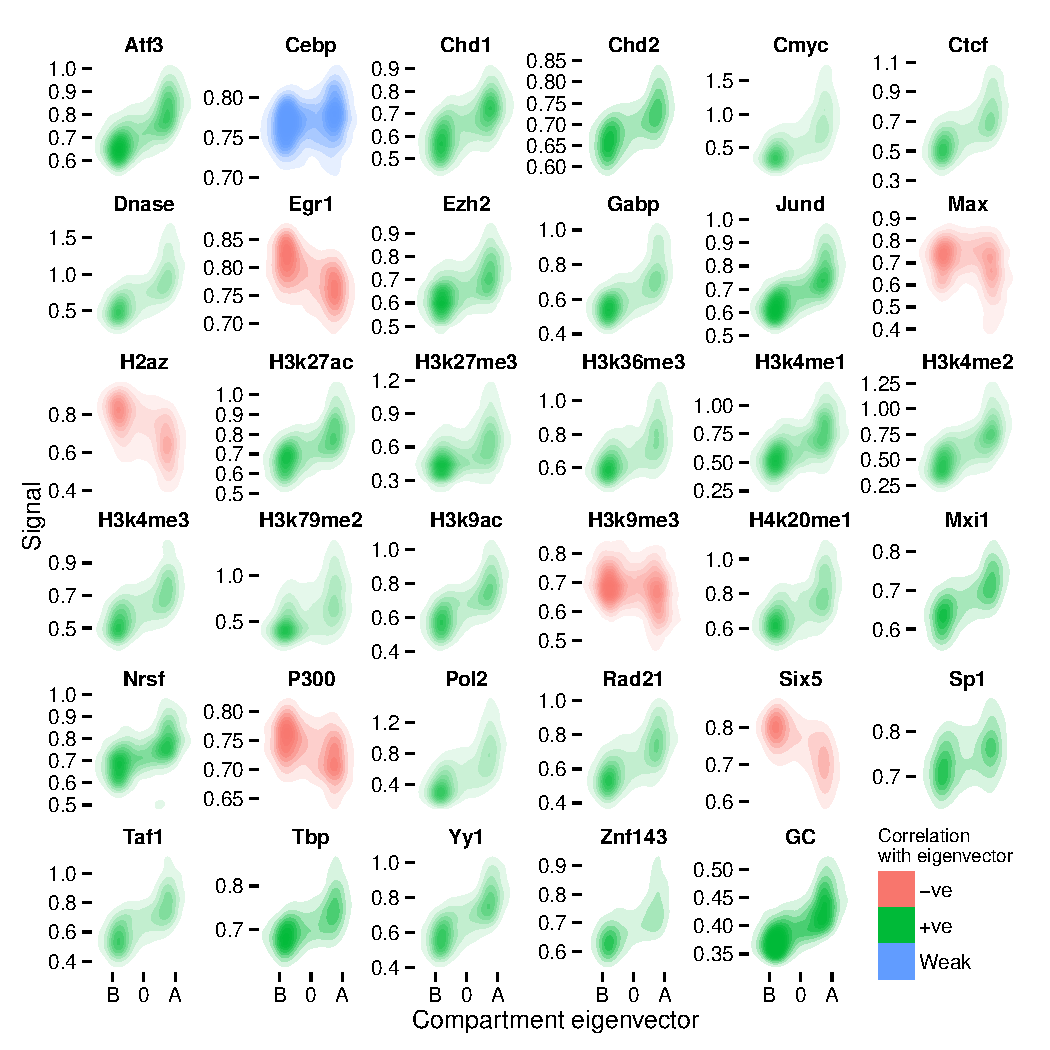
\includegraphics[width=4.5in]{figs/h1feats.pdf}
\captionsetup{width=\textwidth} 
\caption[Correlations of individual features with compartment eigenvector in the H1 hESC cell type.]{ {\bf Correlations of individual features with compartment eigenvector in the H1 hESC cell type. }
Two-dimensional kernel density estimates show the density of points in a scatterplot of compartment eigenvector ($x$-axis) against each input feature individually ($y$-axes). Features with a PCC against eigenvector of above or below $0.1$ are coloured as positive or negative, respectively.
}\label{fig:h1feats}
\end{center} 
\end{figure} 

\begin{figure}
\begin{center} 
\makebox[\textwidth][c]{ 
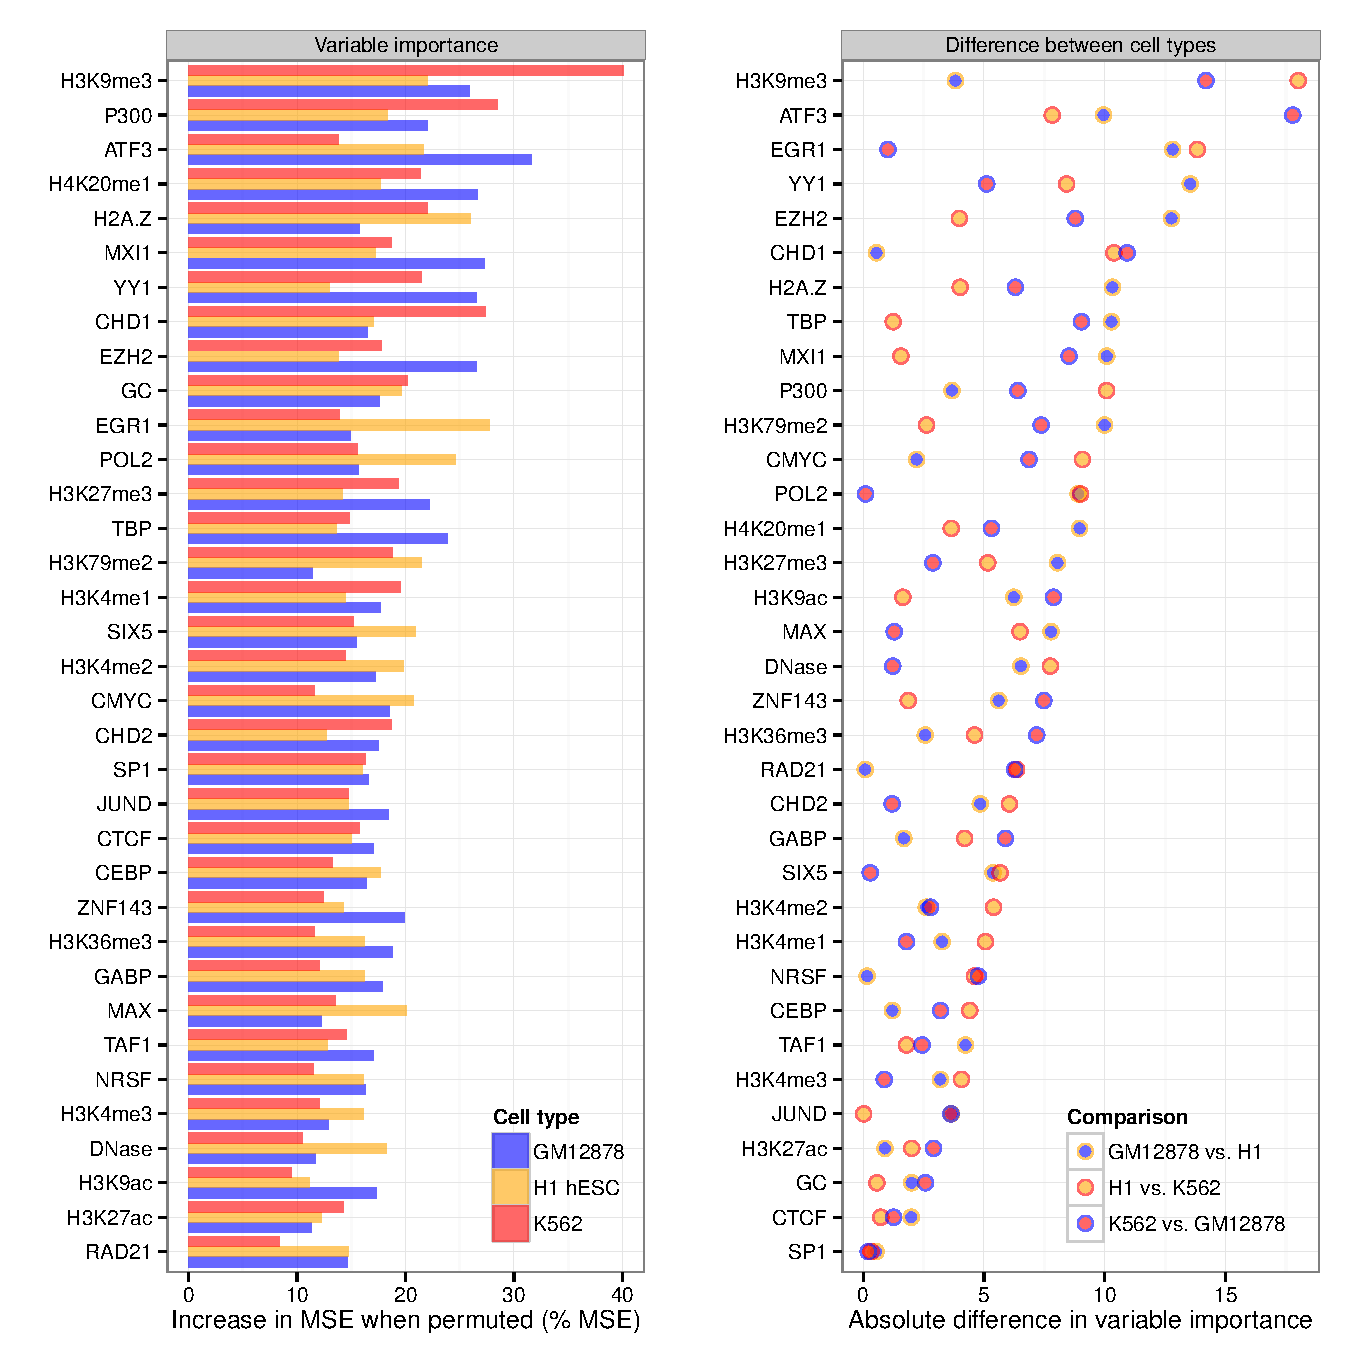
\includegraphics[width=1.1\textwidth]{figs/varimp_diff.pdf}
}
\captionsetup{width=\textwidth} 
\caption[Comparison of variable importance between three cell type specific Random Forest models.]{ {\bf Comparison of variable importance between three cell type specific Random Forest models. }
Variable importance for each Random Forest model was measured in terms of percentage increase in mean squared error when permuted (Methods \ref{sec:rf}). Results are shown sorted by mean variable importance (\emph{left}) and by largest absolute difference in pairwise comparisons (\emph{right}).
}\label{fig:varimp_diff}
\end{center} 
\end{figure} 

In addition to rankings, raw variable importance metrics can be compared between cell-type specific models (Fig. \ref{fig:varimp_diff}). This shows that variables such as CTCF have a relatively small but highly consistent variable importance across the three cell type specific models, whereas other features like ATF3 are highly influential in one cell type but not the other two. Absolute differences in these figures should not be over interpreted and will be affected to some degree by data quality, eigenvector calculation and other sources of noise. Nevertheless there are observations which may reflect biological phenomena, such as the higher relative importance of P300 in both hematopoietic cell line models, potentially reflecting its activity as a histone acetyl transferase that regulates hematopoiesis\cite{Sun2015} and a noted involvement with CTCF in chromatin looping.\cite{Handoko2011}

% also consider looking at LOCAL variable importance

\subsection{Correlating input features}\label{sec:corrinputs}

We have an \emph{a priori} expectation of multicollinearity in our feature set, for example between those that each broadly correlate with transcriptional activity (including POL2, H3K36me3, GC content). To explore these relationships, we performed unsupervised clustering of our feature sets in each cell type (Fig. \ref{fig:featmap}).

\begin{figure}
\begin{center} 
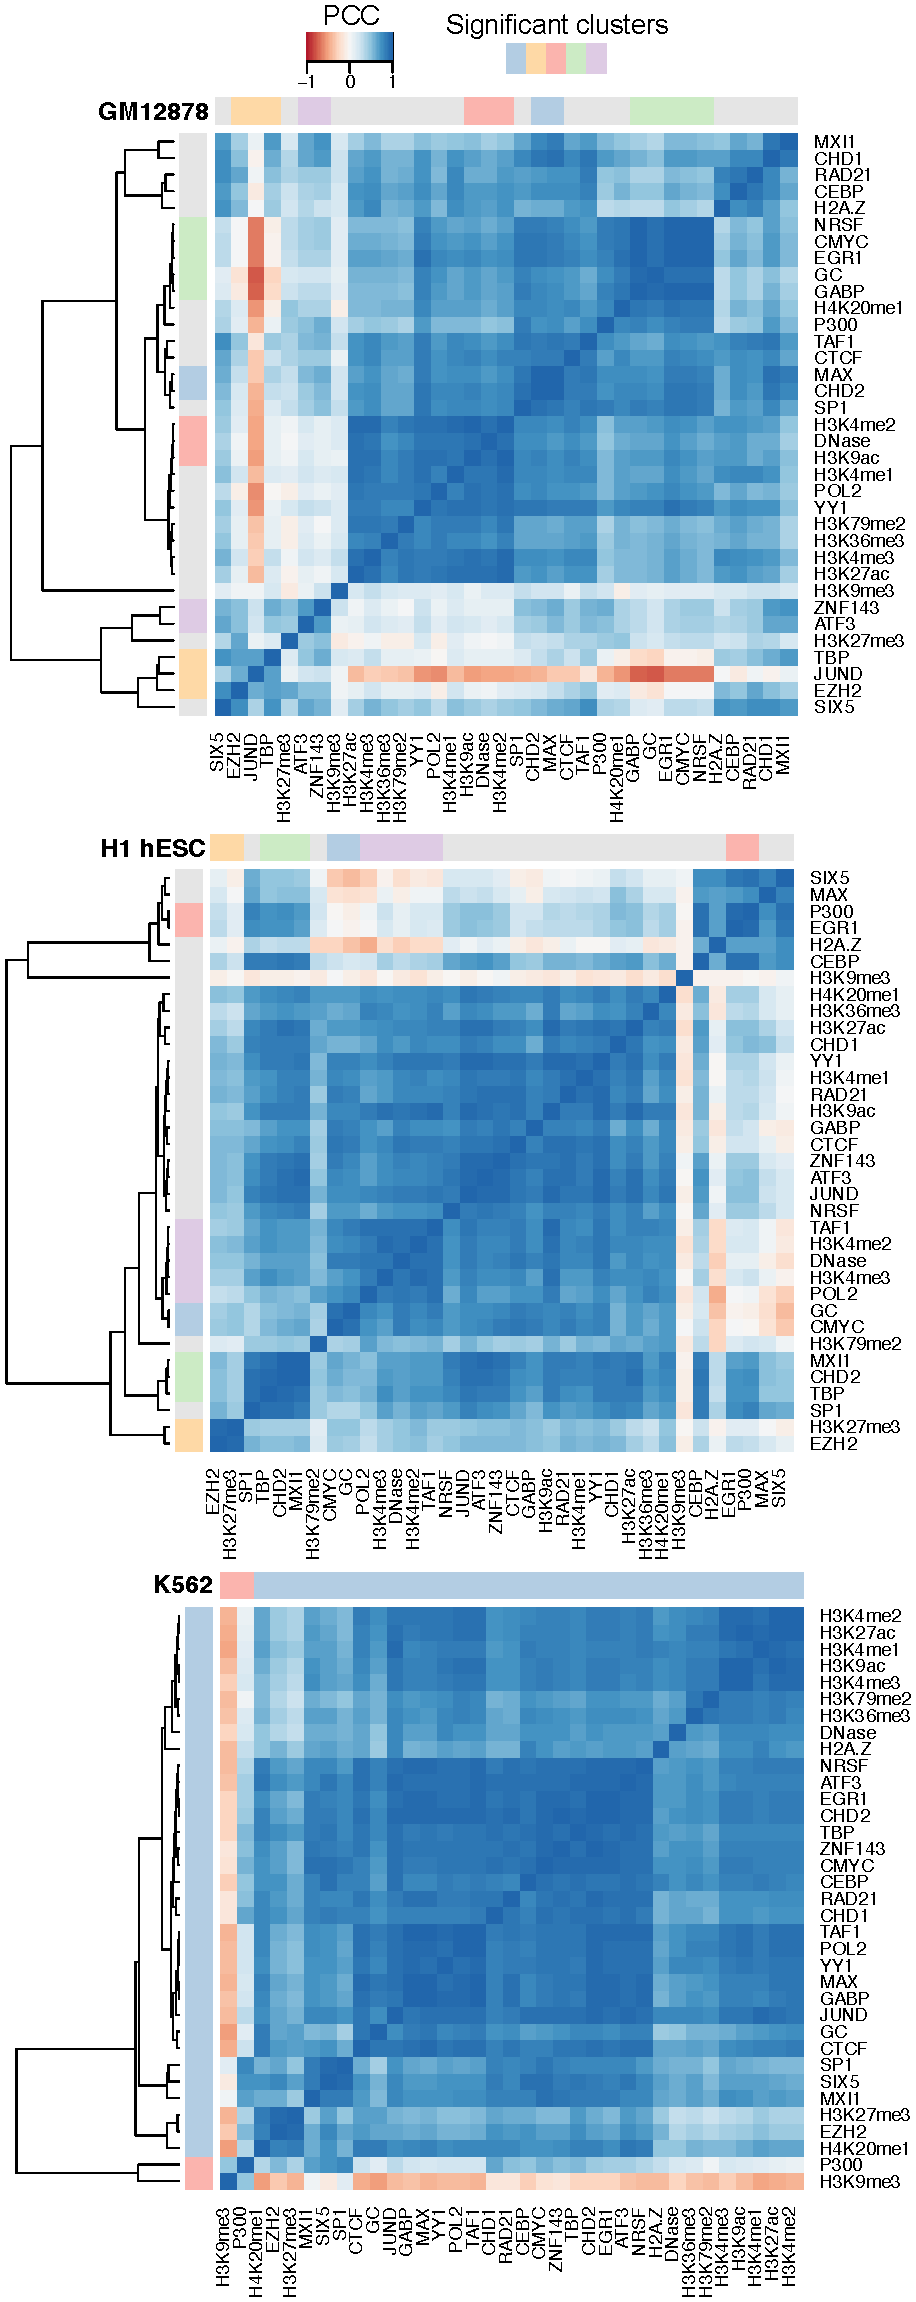
\includegraphics[width=3.6in]{figs/featmap}
\captionsetup{width=\textwidth} 
\caption[Correlation heatmaps of the 35 features used to model compartment eigenvectors.]{ {\bf Correlation heatmaps of the 35 features used to model compartment eigenvectors. }
The Pearson correlation coefficient (PCC) of genome-wide 1 Mb bins of each feature were pairwise correlated with each other. The features were also clustered using hierarchal clustering. The �significance� of these clusters was determined through multi-scale bootstrap resampling, with those clusters that were stable across different sizes of resampling deemed significant, as implemented in the \texttt{pvclust} R package.\cite{Suzuki2006a}
}\label{fig:featmap}
\end{center} 
\end{figure} 

We found pervasive multicollinearity across our feature sets, with the majority of input variables in each model falling into a persistent "active" cluster containing regions with high DNase hypersensitivity, POL2 binding and histone modifications H3K36me3 as well as GC content (Fig. \ref{fig:featmap}). 

Outliers are also present. H3K9me3, noted for high variable importance in each model (Fig. \ref{fig:varimp}) and the only feature ranked within the top 10 in each model (Fig. \ref{fig:top10venn}) is a clear outgroup in the H1 hESC and GM12878 correlation heatmaps, and in K562 forms a stable cluster only with the P300 transcription factor (Fig. \ref{fig:featmap}). This suggests H3K9me3 is providing orthogonal information to many of the other input variables, and likely explains its high variable importance.

\section{Technical considerations}

\subsection{Resolution}

Thus far models were built at 1 Mb resolution, but if we are capturing true biological relationships we would expect these to hold at higher or lower resolutions. To test this, models leaned at 1 Mb resolution were applied to feature sets binned at 100 kb, an order of magnitude higher resolution.

\begin{figure}
\begin{center} 
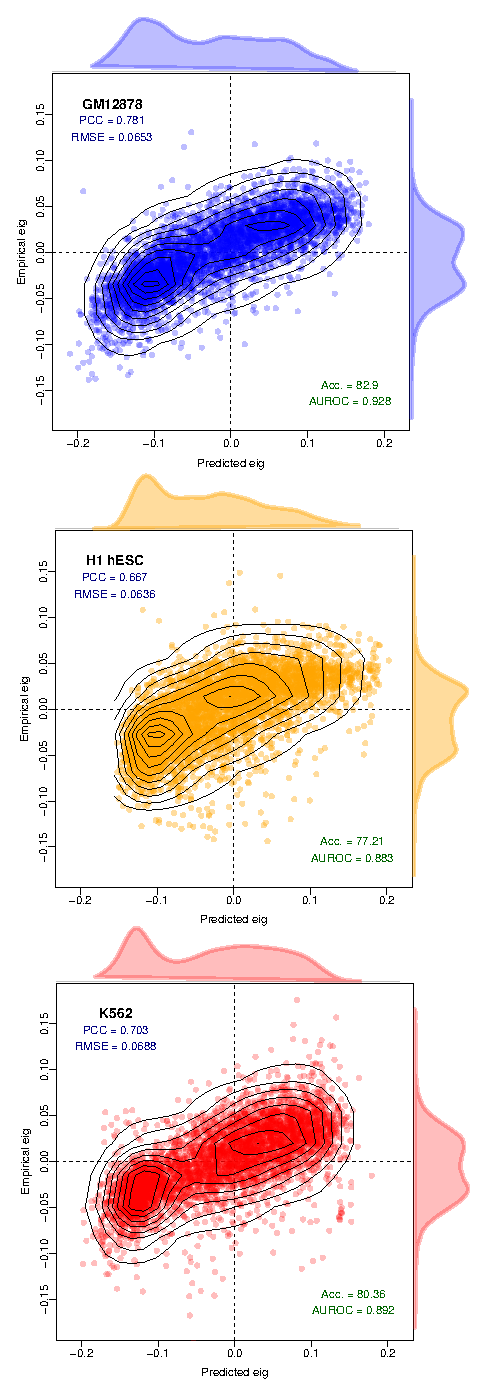
\includegraphics[width=3in]{figs/100kb.pdf}
\captionsetup{width=\textwidth} 
\caption[Models learned at 1 Mb resolution can be applied to higher resolution datasets.]{ {\bf Models learned at 1 Mb resolution can be applied to higher resolution datasets. }
Despite having been trained on low resolution training sets, the Random Forest models generated can successfully predict compartment eigenvectors at higher resolution (100 kb, a $10\times$ zoom). Eigenvectors at a higher resolution than this do not necessarily reflect A/B compartmentalisation.
}\label{fig:100kb}
\end{center} 
\end{figure} 

Model accuracy when applied to higher resolution input features proved to be similarly high, with empirical PCC being $88$ to $95\%$ as high as that at 1 Mb native resolution (Fig. \ref{fig:100kb}).

Note however, there is some indirect leakage between test and training set when 100 kb bins have been used in aggregate in learning the 1 Mb models. Nevertheless, sustained accuracy is evidence that our models are not resolution-sensitive, and could likely be applied to higher resolutions than the 1 Mb predominantly used in this work.

\subsection{Other modelling approaches}

Random Forest (RF) was \emph{a priori} chosen as an appropriate and powerful modelling tool for this work. Other methods could have been used and should be compared. Here we compare our RF approach with two other options: multiple linear regression and partial least squares regression (Methods \ref{meth:othermodels}).

\begin{figure}
\begin{center} 
\makebox[\textwidth][c]{ 
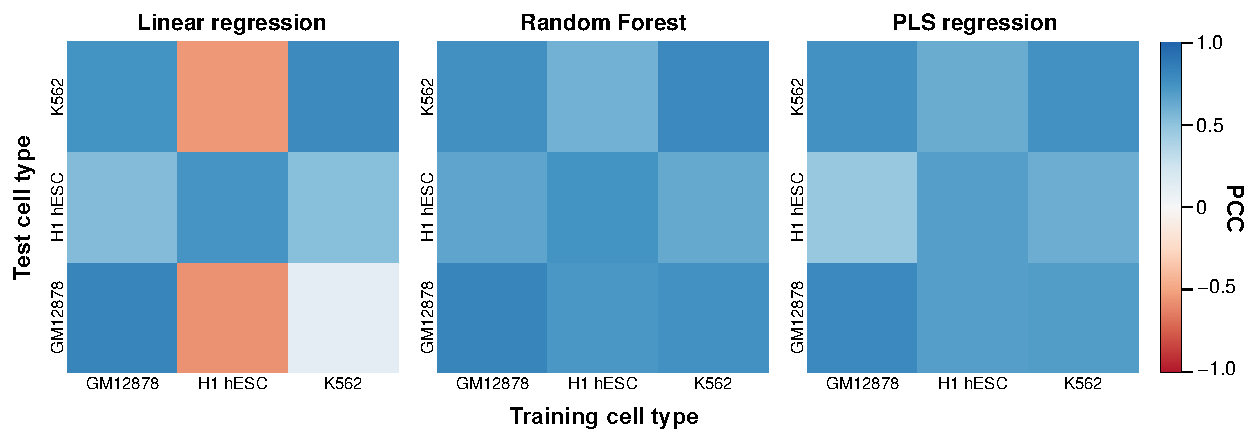
\includegraphics[width=\textwidth]{figs/diffmethods.pdf}
}
\captionsetup{width=\textwidth} 
\caption[Comparison of Random Forest performance with other modelling approaches.]{ {\bf Comparison of Random Forest performance with other modelling approaches. }
Heatmaps show the Pearson correlation coefficient between predicted and observed compartment eigenvectors genome-wide for three regression techniques: multiple linear regression (LM), Random Forest (RF) and partial least squares (PLS). Results are summarised in Table \ref{tab:diffmethods}.
}\label{fig:diffmethods}
\end{center} 
\end{figure} 

Our results confirm RF as a suitable and powerful approach for modelling our relationships of interest in this work (Fig. \ref{fig:diffmethods}), with both the highest cell-type specific performance (PCC between predicted and observed $=0.790$) and on cross-applications (mean PCC $= 0.689$). 

Multiple linear regression assumes linear relationships between model parameters and input features and allows for simple, normally-distributed errors. Surprisingly, this simple approach is capable of accurate cell-type specific predictions (mean PCC $= 0.787$; Table \ref{tab:diffmethods}), likely due to the high raw correlation between the inputs and dependent variable. However this simple approach fails to cross-apply between cell types (mean PCC $=0.139$; Table \ref{tab:diffmethods}) indicating a problems with overfitting. This can be remedied through variable selection procedures, however a strength of the RF approach is that this step is not necessary, and pre-selection of model variables may result in a sub-optimal end result.\cite{Diaz2006}

\begin{table}
\centering
\caption[Performance comparison of different modelling techniques.]{ {\bf Performance comparison of different modelling techniques. }
 Comparison of mean Pearson correlation coefficient between predicted and observed compartment eigenvectors for three different modelling approaches: LM: linear regression; RF: Random Forest regression; PLS: partial least squares regression. Correlations were averaged per cell type over three cell types (cell type specific) and in the six possible crosses (cross-application) shown in Fig. \ref{fig:diffmethods}.
}
\label{tab:diffmethods}
\begin{tabular}{r|ccc}
& {\bf LM} & {\bf RF} & {\bf PLS} \\
\hline
Cell type specific  &  0.787 & 0.790 & 0.750 \\
Cross-application  & 0.139 & 0.689 & 0.641
\end{tabular}
\end{table}

Partial least squares regression is another technique which used dimensionality reduction to engineer a lower-dimension and orthogonal feature set. Hence this method is well-suited to multi collinear inputs, such as the set of variables used in this work (e.g. Fig. \ref{fig:featmap}). As expected, PLS regression provides highly accurate cell type specific predictions (mean PCC $=0.750$; Table \ref{tab:diffmethods}) and during cross-application (mean PCC $=0.641$; Table \ref{tab:diffmethods}), though in both cases produces slightly inferior results to RF models (Fig. \ref{fig:diffmethods}).

PLS uses a type of dimensionality reduction, which offers another way to explore the inter-relationships between our feature set. Plotting input features against these lower-dimension components can give a revelling insight beyond simple correlations (e.g. Fig. \ref{fig:featmap}). Figure \ref{fig:circor} shows a "circle of correlations", where features are plotted onto polar co-ordinates against the first two PLS components (Methods \ref{meth:othermodels}). Interpretation of this figure is that nearby variables in the scatterplot are positively correlated, and the vector length from the circle centre is proportional to said variable's representation in the model. Negatively correlated variables point in opposite directions while uncorrelated variables are orthogonal to each other.\cite{Abdi2010} We therefore see the known multicollinearity represented as groupings of overlapping variables in each cell type, with a smaller number of orthogonal and negatively correlated variables in each cell type (Fig. \ref{fig:circor}).

\begin{figure}
\begin{center} 
\makebox[\textwidth][c]{ 
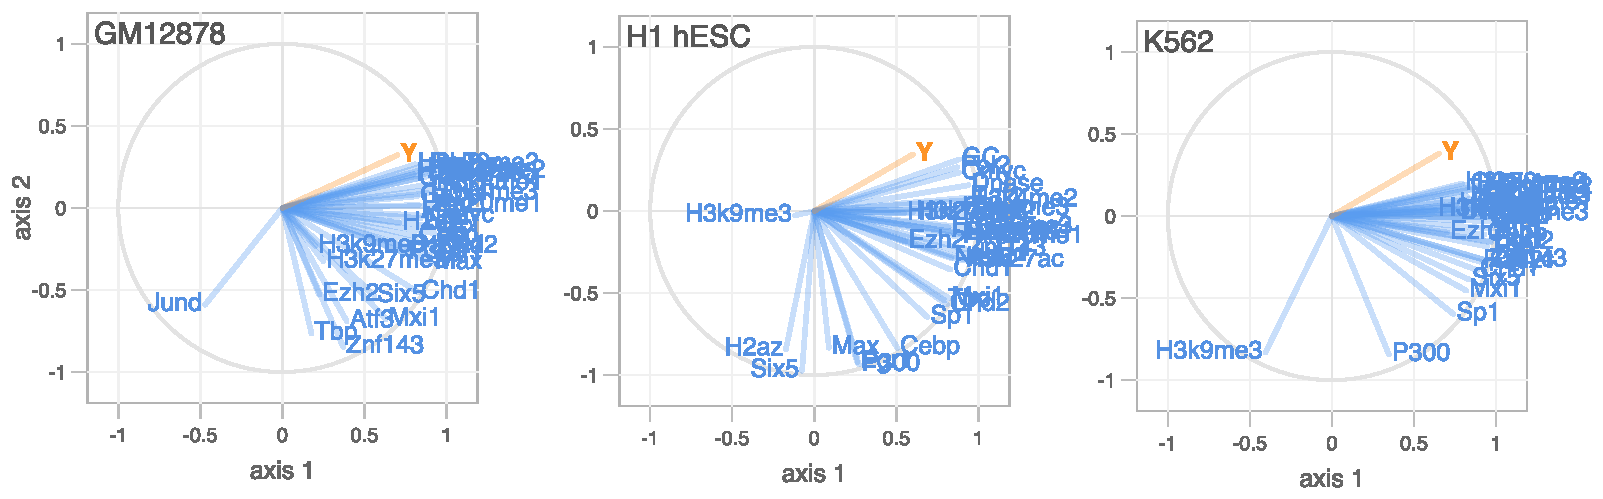
\includegraphics[width=1.1\textwidth]{figs/corcirc.pdf}
}
\captionsetup{width=\textwidth} 
\caption[ Circle of correlations of variables compared with PLS axes. ]{ {\bf Circle of correlations of variables compared with PLS axes.  }
Model variables are plotted against the first two axes used in PLS regression models per cell type. $Y$ represents our compartment eigenvector.
}\label{fig:circor}
\end{center} 
\end{figure} 

\subsection{Non-independence}

% use n-1, n-2, ... as predictors for bin N

As recognised through our use of Hidden Markov Models (Methods \ref{sec:compartments}), consecutive bins along a chromosome are non-independent yet thus far predictive models have not considered this inter-dependence. 

This is for two reasons: firstly non independence could be thought of as an artefact of bin-sizing (we have elected to use regular, fixed binning beneath the scale of compartments themselves whereas another approach could use variable bin sizes, for example per compartment, TAD or restriction fragment); secondly using information of a bin's surroundings may obscure by proxy the chromatin features which would otherwise prove predictive. As an example, knowing that bin $x_{i-1}$ and bin $x_{i+1}$ are in compartment state A would allow us with high confidence to predict the state of bin $x_i$, but without learning anything of the region's relationship with its encompassed histone modifications and bound factors.

\section{Parsimonious models from expanded feature sets}

Strongly predictive models can be useful tools to reason about a complex system, however from a researcher's perspective there also exists a trade-off between predictive power and parsimony. Namely simpler models with fewer inputs may be more interpretable and of wider utility, for example in cell types with less ChIP-seq data available than those used in this work. For this reason we explore parsimonious models with reduced feature sets, with an aim to build simpler models of chromatin state while retaining, if possible, similar levels of predictive accuracy.

Conversely, the $35$ variables used thus far as model inputs are not the complete set available in each cell type, but only the subset of those assayed in all three cell types under study. The ENCODE consortium has produced a significantly greater number of datasets\cite{Dunham2012, Boyle2014} in each cell type which have thus far gone unused. Here we'll explore models of higher order chromatin structure, in some cases built from over $100$ variables, and then generate parsimonious models using optimal subsets guided by statistical techniques that penalise model complexity.

\subsection{Stepwise regression}
% BIC penalised linear models
Multiple linear regression is a simple and analytically well-described modelling framework which is amenable to regularisation through a variety of methods. A simple approach is to start with a complete model and serially remove and/or add variables, then calculate a metric (here we use the Bayesian information criterion, BIC) which weighs the the model likelihood against model complexity. This process is iterated until the metric reaches a (local) minimum, thus creating a more parsimonious model which retains predictive accuracy and should be less prone to overfitting. Stepwise regression also aids interpretation by selecting representative features from collinear clusters.\cite{Mantel1970} A detailed explanation of this feature selection procedure can be found in Methods \ref{meth:stepregress}. It should be noted that despite its continued widespread usage, several statistical issues have been identified with the stepwise procedure for model selection.\cite{Hurvich1990, Whittingham2006}

In terms of model performance alone, stepwise regression gives the highest predictive accuracy on a held-out validation set in each cell type specific model of compartment eigenvector (Table \ref{tab:bicmodels}), however it must be said that differences in model performance across all comparisons are modest. These results do show that even expanded feature sets of up to 187 input features add little explanatory power beyond that of much less complex models with 20 or fewer input variables (Table \ref{tab:bicmodels}). 

% figure: variable importance per linear model

\begin{table}[]
\centering
\caption[Performance comparison of full and optimised RF and ML models.]{ {\bf Performance comparison of full and optimised RF and ML models.}
PCC between predicted and empirical compartment eigenvectors is shown for a range of modelling scenarios, including multiple linear regression (LM) and Random Forest (RF) approaches. For model selection, two methods are used: stepwise BIC-regularised linear models and LASSO regression; in each case those same features were then also used in building a separate RF for comparison.
}
\label{tab:bicmodels}

\makebox[\textwidth][c]{ 
\begin{tabular}{llllllllll}
\multirow{2}{*}{} & \multicolumn{3}{c}{GM$12878$} & \multicolumn{3}{c}{H$1$ hESC} & \multicolumn{3}{c}{K$562$} \\ \cline{2-10} 
 & \multicolumn{1}{|r|}{n} & \multicolumn{1}{c}{LM} & \multicolumn{1}{c|}{RF} & \multicolumn{1}{r|}{n} & \multicolumn{1}{c}{LM} & \multicolumn{1}{c|}{RF} & \multicolumn{1}{r|}{n} & \multicolumn{1}{c}{LM} & \multicolumn{1}{c|}{RF} \\ \hline
\multicolumn{1}{|l|}{All features} & \multicolumn{1}{r}{115} & .836 & \multicolumn{1}{l|}{.828} & \multicolumn{1}{r}{71} & .744 & \multicolumn{1}{l|}{.755} & 187 & .811 & \multicolumn{1}{l|}{.813} \\
\multicolumn{1}{|l|}{Matched subset} & \multicolumn{1}{r}{35} & .827 & \multicolumn{1}{l|}{.823} & \multicolumn{1}{r}{35} & .740 & \multicolumn{1}{l|}{.747} & \multicolumn{1}{r}{35} & .796 & \multicolumn{1}{l|}{.799} \\ 
\multicolumn{1}{|l|}{LASSO $\ell_1$} & \multicolumn{1}{r}{23} & .823 & \multicolumn{1}{l|}{.836} & \multicolumn{1}{r}{23} & .734 & \multicolumn{1}{l|}{.750} & \multicolumn{1}{r}{39} & .779 & \multicolumn{1}{l|}{.811} \\
\multicolumn{1}{|l|}{Stepwise BIC} & \multicolumn{1}{r}{21} & .840 & \multicolumn{1}{l|}{.831} & \multicolumn{1}{r}{13} & .746 & \multicolumn{1}{l|}{.738} & \multicolumn{1}{r}{27} & .819 & \multicolumn{1}{l|}{.810} \\  \hline
\end{tabular}
}
\end{table}

\subsection{LASSO regression}\label{sec:lassoreg}

A more modern technique for regularisation of linear models is the least absolute shrinkage and selection operator (LASSO). In brief, the LASSO is a form of $\ell_1$ regularisation that penalises the sum of absolute values of standardised regression coefficients. By penalising total absolute values, rather than squared values as in $\ell_2$ regularisation, coefficients can be shrunk to $0$ thereby removing terms from the model.\cite{Tibshirani1994, Hastie2001} Thus LASSO combines the coefficient shrinkage of techniques like Ridge regression with a type of feature selection as seen in stepwise regression. A detailed explanation of this method can be found in Methods \ref{meth:lasso}.

Again we can perform a simplistic comparison of model performance using LASSO regression and other techniques (Table \ref{tab:bicmodels}). LASSO retrieves comparable numbers of informative variables to the stepwise regression technique in each cell type, and again removes the majority of input features from expanded sets as redundant or relatively uninformative.

\begin{figure}
\begin{center} 
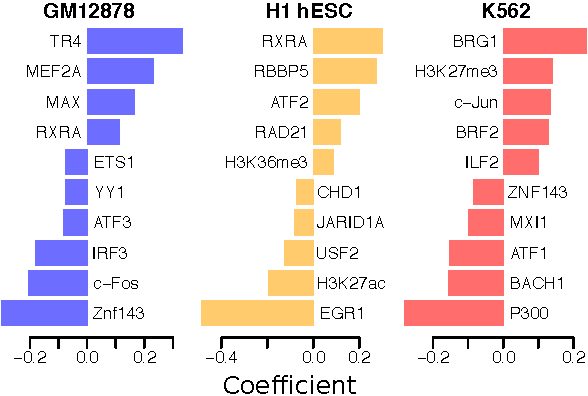
\includegraphics[width=3in]{figs/lasso_bar.pdf}
\captionsetup{width=\textwidth} 
\caption[ Ten largest LASSO model coefficients from expanded feature sets. ]{ {\bf Ten largest LASSO model coefficients from expanded feature sets.  }
Those coefficients with the largest absolute value are plotted for each cell type specific LASSO model. 
}\label{fig:lassobar}
\end{center} 
\end{figure} 

Of those variables with a non-zero coefficient at the optimally-selected tuning parameter $\lambda$ (Methods \ref{meth:lasso}), the ten largest in each cell type are shown (Fig. \ref{fig:lassobar}). Interpretation \ldots XX

% Too many coefficients remain in model for clear plots of coefficient trace
%The LASSO is a tunable algorithm, thus we can gain additional insights of coefficient traces over varying the regularisation parameter, $\lambda$.

\subsection{Regularised Random Forest}

Random Forest (RF) comparisons are included for comparison in Table \ref{tab:bicmodels} where RF models were built using model-selection procedures based on linear regression. The result of this is the linear regression-based feature selection acts as a "filter" method for feature selection, fully independent of the RF learning algorithm. A more coherent approach might be an "embedded" method, where a regularisation procedure is integrated with the learning algorithm.\cite{Guyon2003, Kohavi1997a} %( cite noble review? elements of stat learn?)

While RF is a much younger technique than linear models, a framework for Regularised Random Forests (RRF) has recently been described\cite{Deng2012} and implemented in the R package \texttt{RRF}.\cite{Deng2013a} The RRF algorithm uses the idea that at each node in a tree, unused variable should only be included if they offer a significant information gain over those available variables which have already been used in the tree. This differs from the standard RF algorithm where splitting decisions at each node are entirely independent of each other (Methods \ref{sec:rf}). 

We found that this algorithm was unable to perform feature selection on our highly collinear feature set, instead leaving full or almost full feature sets in each case (\emph{data not shown}) and so providing equal results to a standard RF model using expanded feature sets (Table \ref{tab:bicmodels}).

\ifstandalone
\begin{small}
\bibliography{/Users/benmoore/Documents/library,/Users/benmoore/Documents/customrefs}
\end{small}
\fi

\end{document}
